\chapter{The Shared Annotator Setting}

%\label{sec:setting} 

In our setting, there are $K$  binary classification tasks to be learned simultaneously. 
In opposed to the common multi-task classification settings, here, no dependency between the tasks 
is assumed during the analysis, but the tasks can be dependent as well. 
The model learning is performed in rounds as an online learning algorithm, as following: 
On each round $t$, there are $K$ input-label pairs
$(\vxi{i,t},\yi{i,t})$, one for each classification tast, where $i=1,2\comdots K$ is the task index and $t$ is the 
step index. The inputs $\vxi{i,t}\in\reals^{d_i}$ are vectors, and the labels  $\yi{i,t}\in\{-1,+1\}$ are binary. 
In the general case, the input-spaces for each problem may be different, and inputs may
have different number of elements. Yet, in order to  simplify the notation and without loss of generality,  
from now on, in our analysis we assume that for all of the tasks, $\vxi{i,t}\in\reals^{d}$. 
i.e. all the tasks are in the same dimension and   $d_i = d$ holds for all tasks . 
In practice, since the proposed algorithms use the margin that is affected by the vector norm, 
there is a need to scale all the vectors into a ball.


On round $t$, the learning algorithm receives $K$ input vectors $\vxi{i,t}$
for $i=1 \comdots K$ tasks and produce  $K$  binary-labels output $\hyi{i,t}$, where
$\hyi{i,t}\in\{-1,+1\}$ is the label predicted for the input
$\vxi{i,t}$ of task $i$. The algorithm then chooses a task $J_t \in\
\{1 \comdots K\}$ and asks from an annotator its true-label
$\yi{J_t,t}$ for that task $J_t$. Unlike the usual online multi-task setting, and due to the limitation of our
setting, it  does not observe any other label. 
Then, the algorithm updates its models, using the received feedback, and proceeds to the
next round (and inputs).  For the ease of calculations below, we denote
by $K$ indicators $Z_t=\paren{ Z_{1,t} \comdots Z_{K,t}}$, the
identity of the task which was queried on round $t$, and set
$Z_{J_t,t}=1$ and $Z_{i,t}=0$ for $i\ne J_t$. Clearly from the definition, the condition, $\sum_i
Z_{i,t}=1 ,\forall{i,t}$, always holds . Below, we define the notation $\Expp{t-1}{x}$ to be the
conditional expectation $\Exp{x \vert Z_{1},...Z_{t-1}}$ given all
previous choices of the tasks to be queried.


Schematic illustration of a single iteration of multi-problem algorithms is shown in \figref{fig:ilustration}. The top panel shows the standard
setting of online multi-task algorithms with a shared annotator, that labels all inputs, which are fed to the corresponding algorithms to update corresponding models. The
bottom panel shows the SHAMPO algorithm, which couples labeling
annotation and learning process, and synchronizes a single annotation
per round.  At most one task performs an update per round, the one
with the annotated input.

\begin{figure}
\begin{centering}
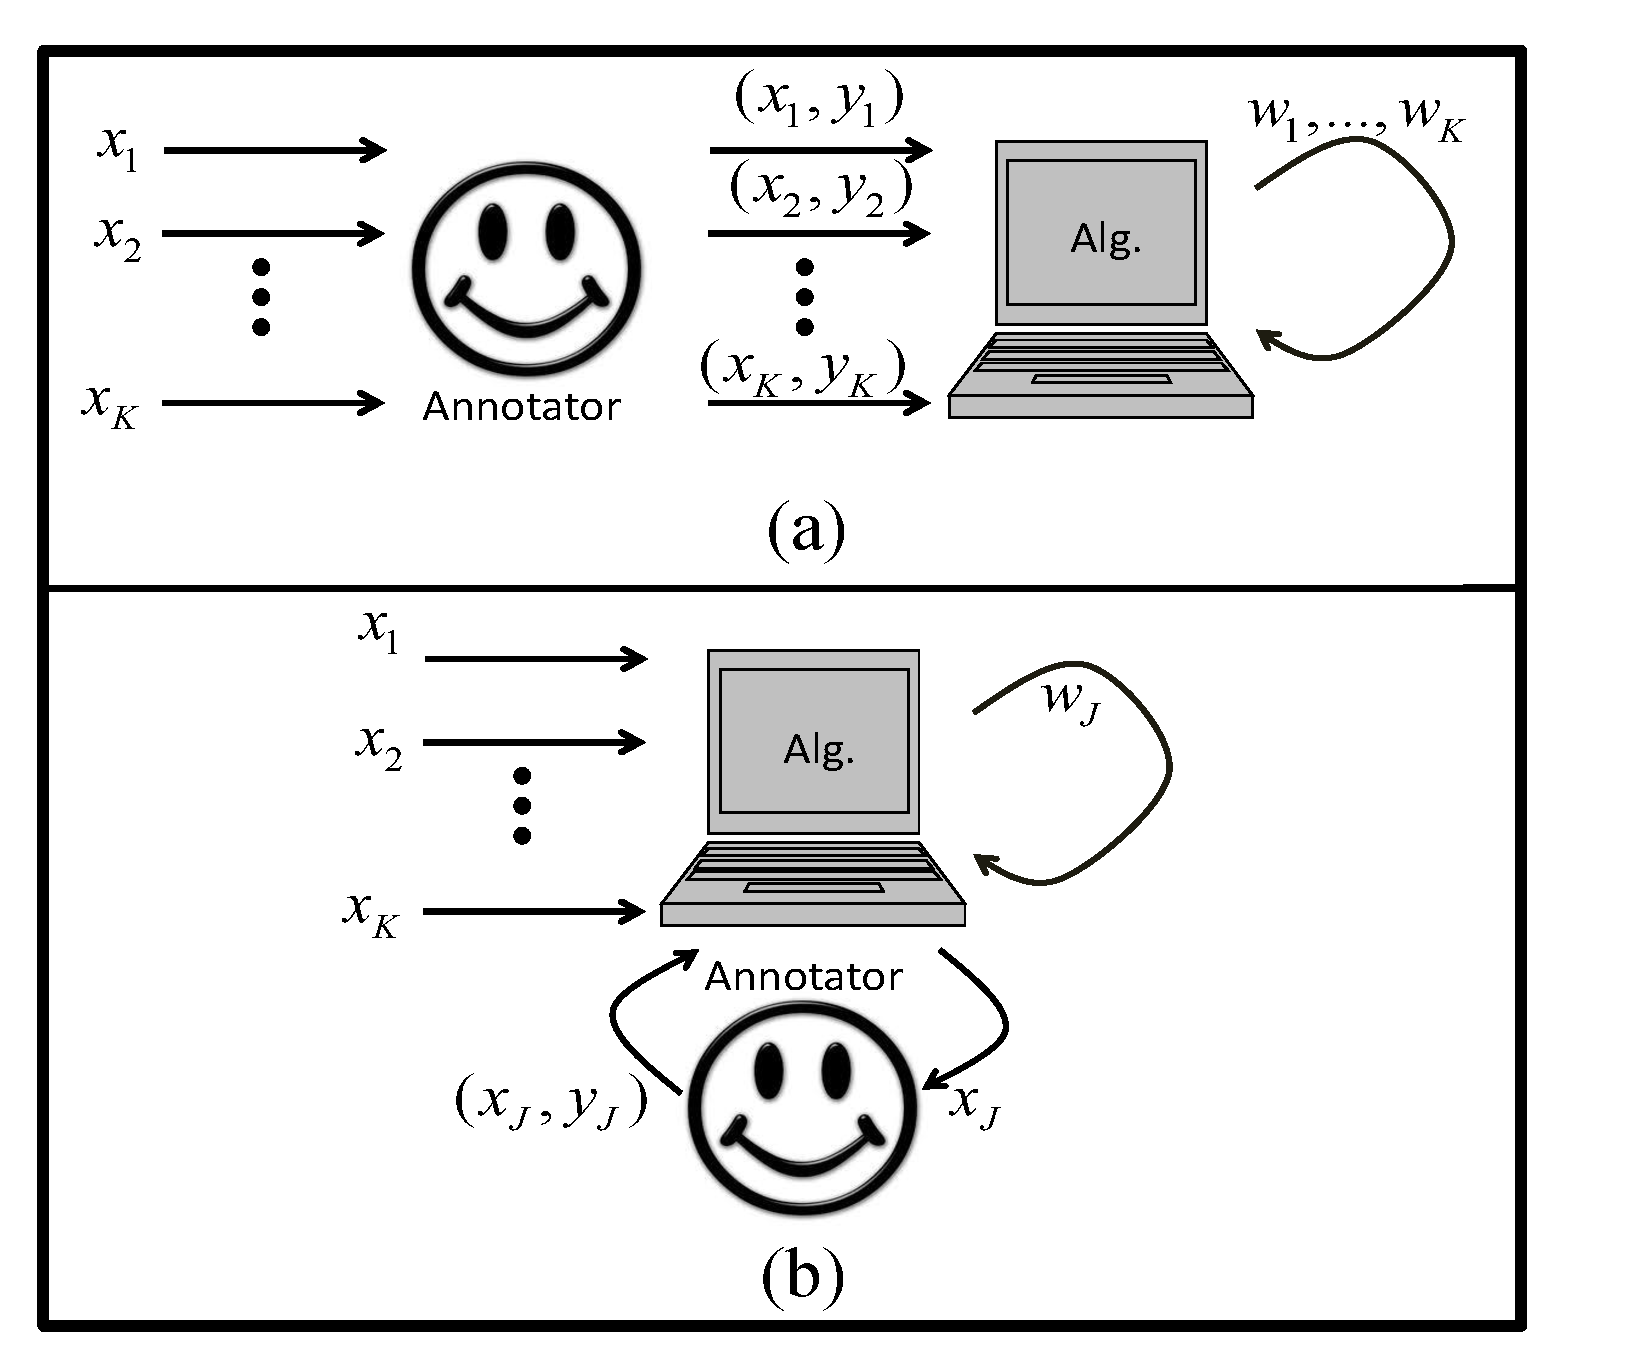
\includegraphics[width=0.5\textwidth]{figs/SHAMPO_illustration.eps}
\caption{Illustration of a single iteration of  multi-task algorithms (a) standard setting, shared annotator labels all inputs, and algorithms update models. (b) SHAMPO algorithm couples labeling annotation and learning process, and synchronizes a single annotation per round.}
\label{fig:ilustration}
\end{centering}
\end{figure}

\begin{figure}
\begin{centering}
\includegraphics[width=0.7\textwidth]{figs/table_ss.eps}
\end{centering} 
%\vspace{10}
\begin{centering}
\includegraphics[width=0.7\textwidth]{figs/table_SHAMPO.eps}
\caption{In selective sampling we focus on when to issue a query for a single task (a row), while in the SHAMPO setting we
   COMPLETE THIS SENTENCE  }
\label{fig:ss_vs_SHAMPO}
\end{centering}
\end{figure}

